\documentclass[11pt]{article}
\usepackage[top=15mm,bottom=15mm,left=15mm,right=15mm]{geometry}
\usepackage{mathptmx}
\usepackage[T1]{fontenc}
\usepackage{fancyhdr}
\usepackage{lastpage}
\usepackage{pgfgantt}
\usepackage{wrapfig}
\usepackage{array, xcolor}
\usepackage{booktabs}
\usepackage{color, colortbl}
\usepackage{hyperref}
\definecolor{lightgray}{gray}{0.8}
\newcolumntype{L}{>{\raggedleft}p{0.21\textwidth}}
\newcolumntype{R}{p{0.75\textwidth}}
\newcommand\VRule{\color{lightgray}\vrule width 0.5pt}
\newcommand{\todo}[1]{{\scriptsize\color{red}TODO:#1}}
\newcommand{\ul}{\underline}
\usepackage[font=footnotesize,labelfont=bf]{caption}
\parindent=0pt
\pagestyle{fancy}
\fancyhf{}
\usepackage{wrapfig}
\usepackage{csquotes}

\usepackage{multicol}
\usepackage{titlesec}
\titlespacing\section{0pt}{5pt plus 2pt minus 2pt}{5pt plus 2pt minus 2pt}
\titlespacing\subsection{0pt}{5pt plus 2pt minus 2pt}{5pt plus 2pt minus 2pt}
\titlespacing\subsubsection{0pt}{5pt plus 2pt minus 2pt}{5pt plus 2pt minus 2pt}

\usepackage{multicol}

\fancyfoot[c]{\color{gray}\small Dr. Werner Dobrautz $\vert$ \href{mailto:werner.dobrautz@gmail.com}{werner.dobrautz@gmail.com} $\vert$ \href{https://dobrautz.github.io/}{dobrautz.github.io}}

%\fancyfoot[C]{\footnotesize Part B2 -- Page \thepage$\;$of$\;$ \pageref{LastPage}}


%\fancyfoot[C]{{\setlength{\fboxrule}{0.5pt}
		%		\fcolorbox{black}{black!20}{\hfill \footnotesize Part B2 -- Page \thepage$\;$of$\;$ \pageref{LastPage}}}
	%}

\setcounter{section}{3}

\renewcommand{\headrulewidth}{0.0pt} %obere Trennlinie
\setcounter{secnumdepth}{2}

%opening
\title{MSCA -- Part B2}
\author{Werner Dobrautz}

\title{\bfseries\Huge Werner Dobrautz}
\author{werner.dobrautz@gmail.com}
\date{}

\begin{document}
	%\thispagestyle{empty}
	
	\vspace*{-2cm}
	\begin{center}
		\huge \bf Curriculum Vitae -- Dr. Werner Dobrautz
	\end{center}
	
	%\section*{Personal and Contact Information}
	\vspace*{-0.35cm}
	
	\begin{tikzpicture}
		\node[] (1) {
		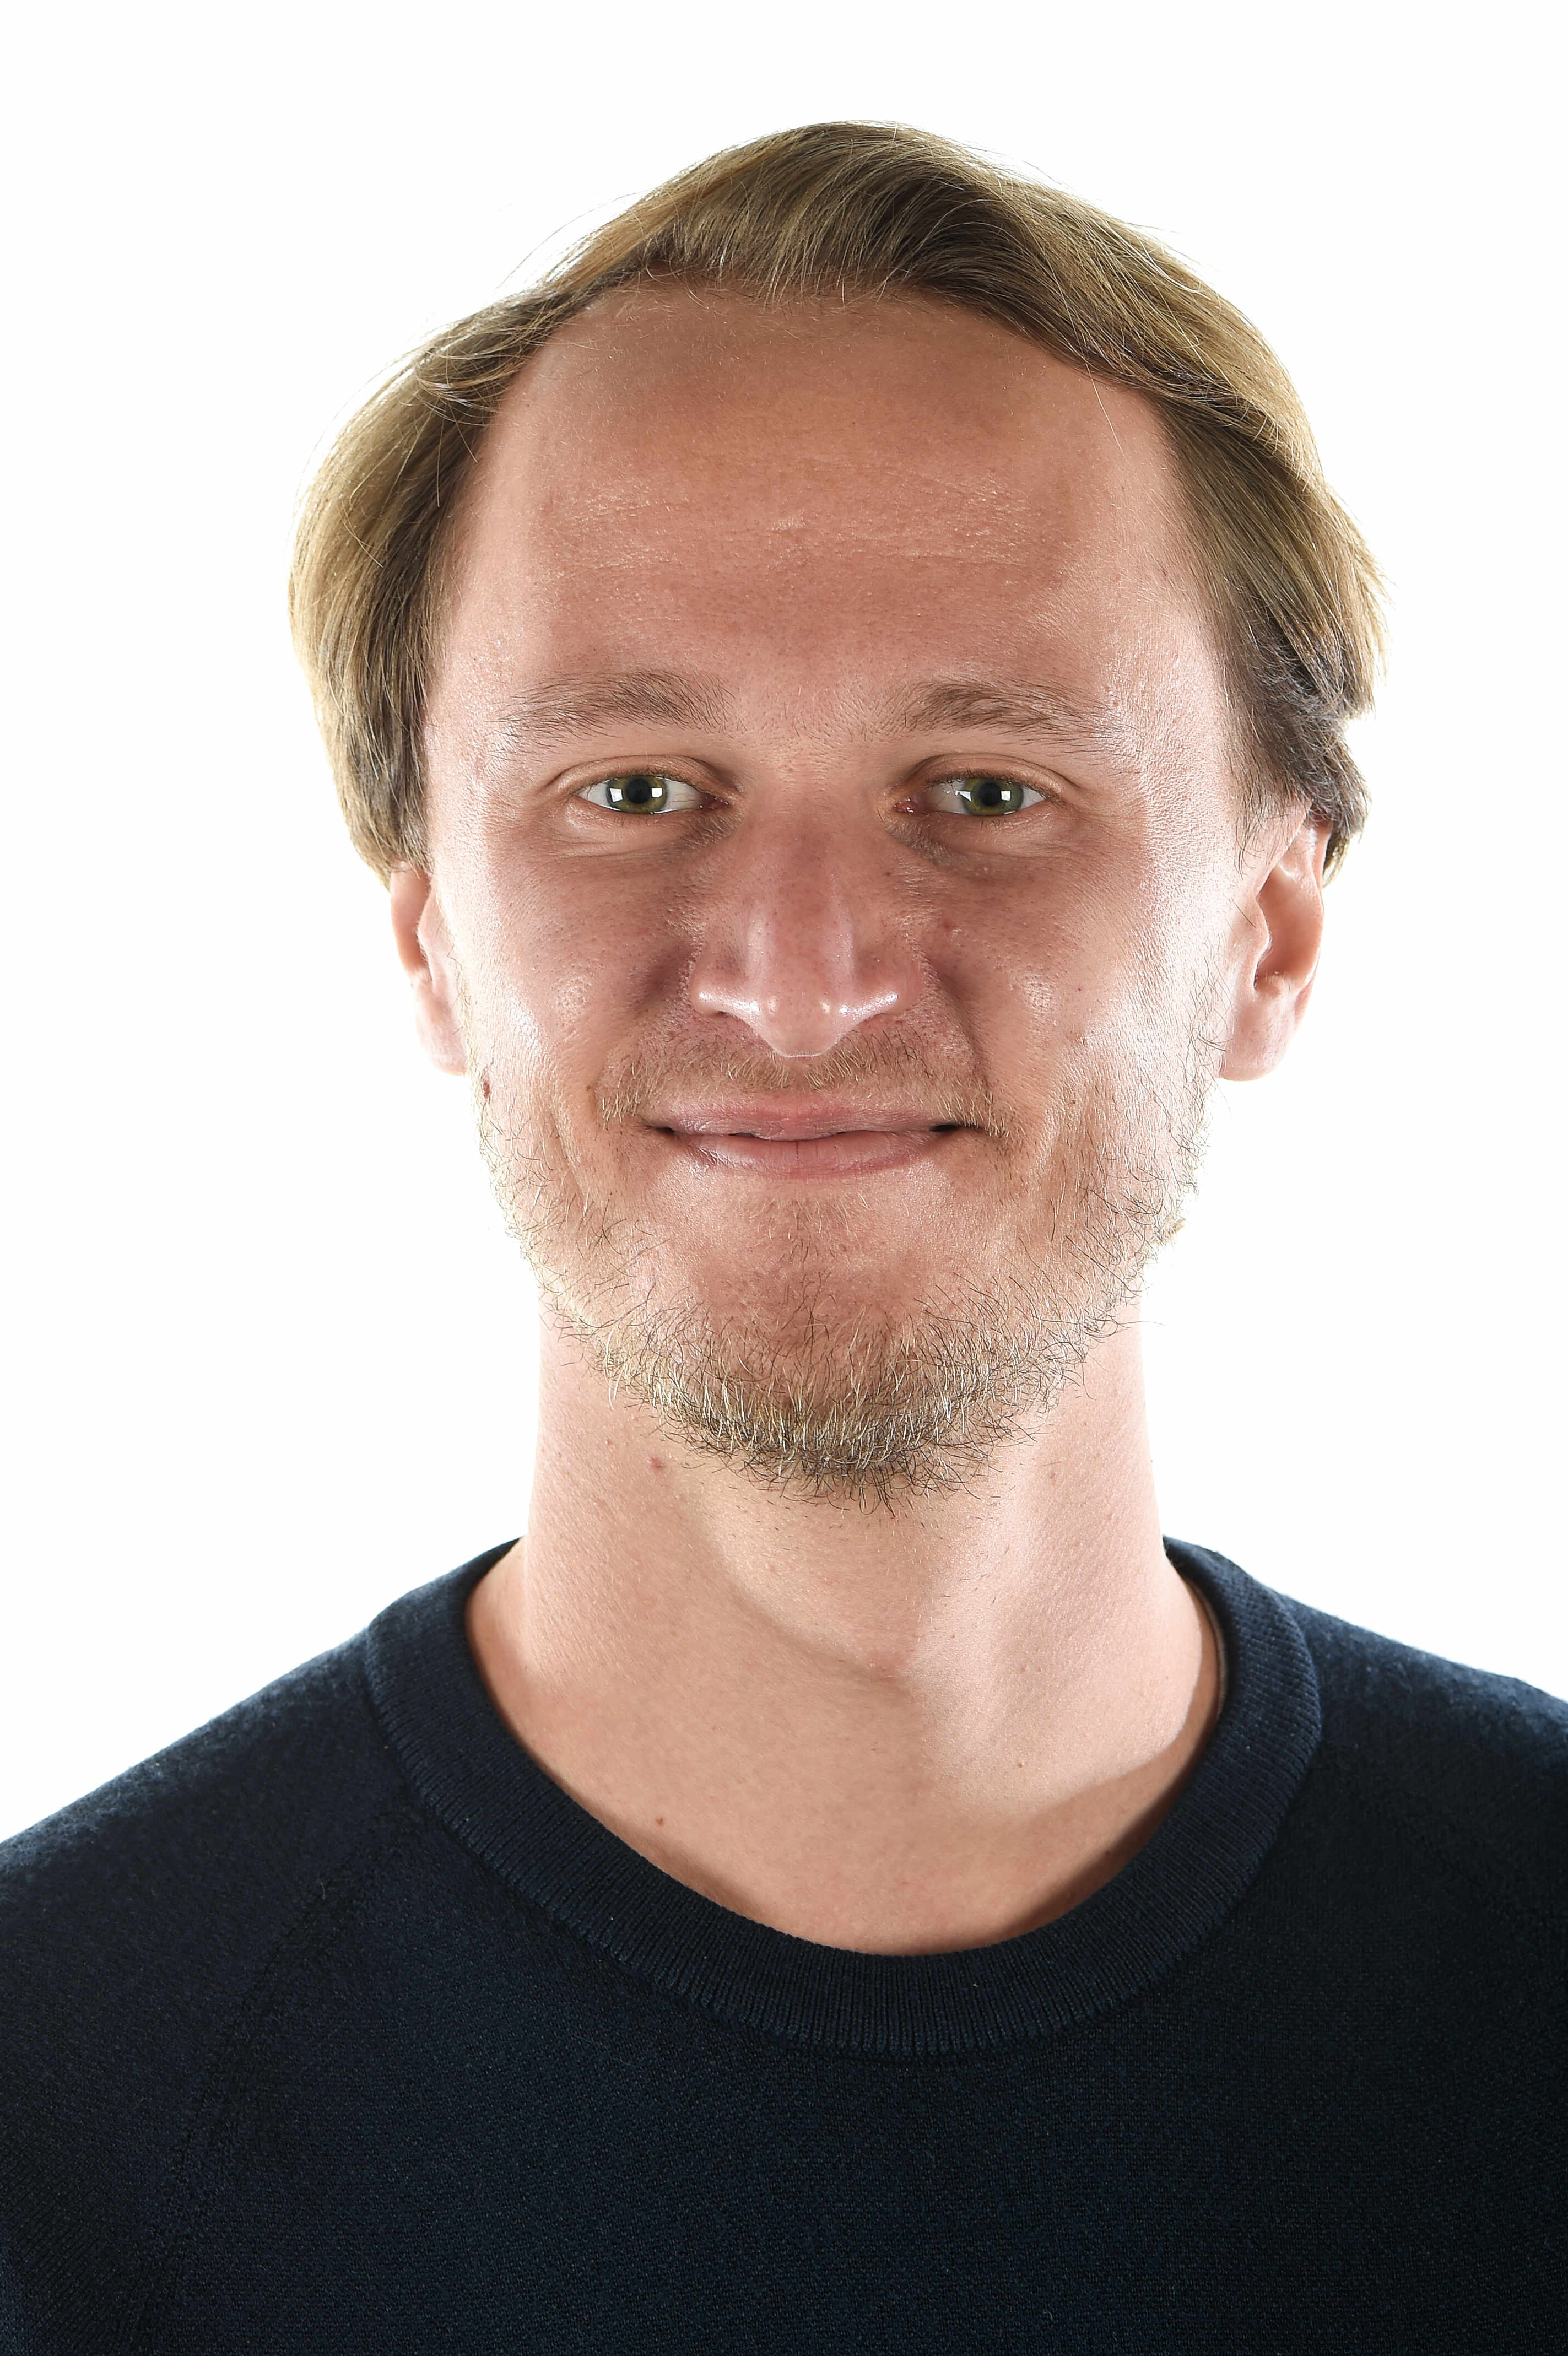
\includegraphics[height=4cm]{WDobrautz-4-comp}
	};
\node[right=1.5cm] at (1.east) {
\begin{minipage}{0.8\textwidth}
	\begin{center}
	\begin{tabular}{ll}
		Full Name: & Werner Dobrautz \\
		Date of birth: & 02.11.1987 \\
		%Nationality: & Austrian \\
%		Phone number: & +49 163 5133042 \\
		E-mail: & \href{mailto:werner.dobrautz@gmail.com}{werner.dobrautz@gmail.com}\\
%		Private Address: & Barken Beatrices Gata 16, 41760 Gothenburg, Sweden \\
		Work Address: & Chalmers University of Technology, \\ & Department of Chemistry and Chemical Engineering, \\ &Kemigården 4, SE-412 96 Göteborg, Sweden \\
		Research IDs: &  
		\href{https://scholar.google.de/citations?user=mTuKWjMAAAAJ&hl=en}{Google Scholar},
		\href{https://orcid.org/0000-0001-6479-1874}{ORCiD: 0000-0001-6479-1874} \\
		Contact/Social Media/Homepage: & \href{https://dobrautz.github.io/}{dobrautz.github.io}, \href{https://mastodon.cloud/@dobrautz}{Mastodon}, \href{https://twitter.com/dobrautz}{Twitter}, \href{https://www.linkedin.com/in/werner-dobrautz-46873a190/}{LinkedIn}
	\end{tabular} 
\end{center}
\end{minipage}
};
	\end{tikzpicture}

	
%	\vspace*{0.3cm}
%	\section*{Personal Statement}
	
	\begin{wrapfigure}[10]{r}{0.3\textwidth}
		\vspace{-0.8cm}
		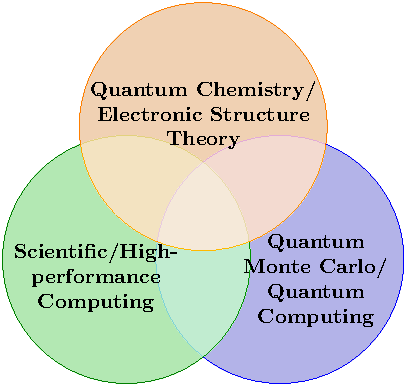
\includegraphics[width=0.28\textwidth]{venn}
	\end{wrapfigure}
	
	
	After a graduate study of physics, with specialization in computational solid state physics, and a subsequent Ph.D. in computational quantum chemistry in the
	field of stochastic wavefunction theory for strongly correlated electron systems,
	I am currently a Marie Skłodowska-Curie Postdoctoral Fellow at Chalmers University of Technology 
	developing novel quantum computing algorithms to perform realistic \emph{ab initio} calculations on 
	near-term quantum computing devices.
	I have strong knowledge of a variety of modern theoretical and computational quantum chemistry methods and I acquired
	extensive algorithm design and development expertise as the main developer of the publicly available quantum Monte
	Carlo code \href{https://github.com/ghb24/NECI_STABLE}{\texttt{NECI}} during my Ph.D. and consequent PostDoc.
	
	The two main areas of my research are the \textbf{(1)} development 
	of novel quantum computing algorithms to perform realistic 
	\emph{ab initio} calculations on 
	near-term quantum computers as well as 
	\textbf{(2)} developing highly accurate 
	quantum Monte Carlo methods for high-performance computing clusters to solve strongly correlated electron problems.
	
	
	\section*{Professional and Academic Research Experiences}
	\renewcommand{\arraystretch}{1.2}
	\begin{tabular}{L!{\VRule}R}
		Since 01.07.2023 & \textbf{Remote Fellow -- \href{https://www.kit.edu/research/yig-prep-pro.php}{Young Investigator Group Preparation Program}}, 
		Karlsruhe Institute of Technology, Steinbuch Centre for Computing,  Karlsruhe, Germany.  \\
		& Preparation and Mentorship Program for Independent Group Leader Funding Applications\\
		Since 01.07.2022 & \textbf{Marie Skłodowska-Curie Postdoctoral Fellow}, Chalmers University of Technology and Wallenberg Centre for Quantum Technology, Gothenburg, Sweden  \\
		& Quantum algorithm development to enable accurate and efficient \emph{ab initio} calculations on current and near-term quantum computers \\
		01.10.2021 -- 30.06.2022 & \textbf{Postdoc}, Chalmers University of Technology, Gothenburg and IBM Academic Network \\
		& Development of novel quantum computing algorithms to perform realistic \emph{ab initio} calculations on 
		near-term quantum computing devices \\
		01.04.2019 -- 30.09.2021 & \textbf{Postdoc}, Max Planck Institute for Solid State Research, Stuttgart, Germany \vspace{-0.2cm}
		\begin{itemize} \itemsep0em 
			\item Development of highly accurate quantum Monte Carlo methods for strongly correlated electron systems. Application to solid-state model Hamiltonians and strongly correlated bio-chemical transition-metal clusters.
			\item Development of highly optimized massively parallel algorithms for high-performance computing centers.
			\item Collaboration with industry partners to enable accurate quantum chemical calculations on NISQ 
			quantum computing devices.
		\end{itemize}\\[-8pt]
		01.09.2020 -- 30.06.2021 & \textbf{Math Teacher} at \emph{Haus der Lebenschance}, eva e.V, Stuttgart, Germany \\
		& Teaching math for adults attempting to catch up on graduation (6h / week)\\
		01.10.2012 -- 30.09.2014 & \textbf{University Project Assistant}, Graz University of Technology, Graz, Austria \\
		& Tutor in  \emph{Quantum Mechanics}, \emph{Theoretical Electrodynamics}, \emph{Advanced Quantum Mechanics} and \emph{Advanced Computational Physics} and development of Monte Carlo methods for strongly correlated electron systems \\
		01.10.2011 -- 30.09.2012 & \textbf{Data analyst} in the field of pharmaceutical process and product design, Research Center Pharmaceutical Engineering GmbH, Graz, Austria 
	\end{tabular}
	
	\section*{Academic Studies}
	\renewcommand{\arraystretch}{1.3}
	\begin{tabular}{L!{\VRule}R}
		01.11.2014 -- 26.03.2019 & \textbf{Ph.D.} (Dr.\,rer.\,nat.) in theoretical quantum chemistry (\emph{summa cum laude}), MPI for Solid State Research and University of Stuttgart, Germany, Ph.D. award date: 26.3.2019 \\
		& Thesis: \emph{Development of full configuration interaction quantum Monte Carlo (FCIQMC) methods for strongly correlated electron systems}, Supervisor: Prof. Ali Alavi\\
		01.10.2011 -- 28.03.2014 & \textbf{MSc} (Dipl.-Ing.) in Technical Physics (\emph{with distinction}), Graz University of Technology, Focus: Theoretical and Computational Physics, Graz, Austria, MSc award date: 28.3.2014 \\
		& Thesis:  \emph{Application of the FCIQMC algorithm to the two-dimensional fermionic Hubbard model}, Supervisor: Prof. Wolfgang von der Linden \\
		01.10.2007 -- 11.04.2011 & \textbf{BSc} in Technical Physics, Graz University of Technology, Graz, Austria \\
	\end{tabular}	
	
	\subsection*{Schools and Workshops}
	
	%\newcolumntype{L}{>{\raggedleft}p{0.1\textwidth}}
	%\newcolumntype{R}{p{0.85\textwidth}}
	\renewcommand{\arraystretch}{1.3}
	\begin{tabular}{L!{\VRule}R}
		2022 & \textbf{Lecturer} at Winter School in Theoretical Chemistry, \emph{Quantum Computers for Chemistry},  University of Helsinki, Helsinki, Finland  \\
		2021 & Quantum Open Source Foundation -- QOSF -- Mentorship Program \\
		2021 & Qiskit Global Summer School on Quantum Machine Learning \\
		2019 & Advanced C++ with Focus on Software Engineering, HLRS, Stuttgart, Germany \\
		2017 & European Summer School in Quantum Chemistry -- ESQC, Sicily, Italy \\
		2017 & Many Electron Collaboration Summer School of the \emph{Simons Foundation}, Stony Brook University, New York, USA \\
		2017 & AWS Artificial Intelligence Bootcamp, Stuttgart, Germany \\
		2015 & Tensor Network Summer School, Ghent University, Belgium \\
	\end{tabular}	
	
	\section*{Teaching, Pedagogical Experience and Supervision of Students}
%	During my graduate studies at Graz University of Technology, I was employed as a \emph{University Project Assistant} and was working as a \emph{tutor} in the practical part of the courses: \emph{Quantum Mechanics}, 
%	\emph{Theoretical Electrodynamics}, \emph{Advanced Quantum Mechanics} and \emph{Advanced Computational Physics}. 
%	My duties involved holding and grading the exercise classes, which also entailed giving various lectures on 
%	specific topics not covered in the main lecture class. 
%	Additionally, we were tasked with designing and grading the intermediate and final written exams in these courses. 
%	
%	From September 2020 until July 2021, I was working as a math teacher at the charitable institution \emph{Haus der Lebenschance} of the \emph{Evangelische Gesellschaft (eva) e.V.}, which helps young adults, often with troublesome and/or migration backgrounds, without any graduation to catch up on education. 
%	I was working there 6 hours per week, and my duties consisted of holding the math lectures (6 $\times$ 45min) and
%	conceiving homework \& mock exams and grading them. 
%	
%	
%	I am currently obtaining the Swedish \emph{Diploma in Teaching and Learning in Higher Education} and as a part of it I recently completed the \emph{University Teaching and Learning} course at Chalmers University
	
	%	{\color{red}\bf add Erika Master info}
	
	\vspace{0.5cm}
	\renewcommand{\arraystretch}{1.2}
	\begin{tabular}{L!{\VRule}R}
		\hline
		\rowcolor{black!20}
		\multicolumn{2}{c}{\bf	\large Supervision of students} \\
		\hline
%		2019 -- 2021  & Co-supervision of a Ph.D. student at the MPI Stuttgart \\
		2021 -- now & Co-supervision of a Ph.D. student at Chalmers University \\
		2022 & Supervision of two students in Physics Master course project \emph{Building and programming a quantum computer} at Chalmers University \\
		Jan. 2023 -- June 2023 & Supervision of a Master student at Chalmers University \\
		\bottomrule
	\end{tabular}
	
%	\newpage
	\begin{center}
		\bf	\Large Lectures
	\end{center}
	\vspace*{-0.5cm}
	\begin{center}
		\renewcommand{\arraystretch}{1.1}
		\begin{tabular}{p{0.09\textwidth}p{0.35\textwidth}p{0.19\textwidth}p{0.1\textwidth}c}
			\hline
			\rowcolor{black!20}
			Year & Subject & Degree &  Type & Week hours \\
			\hline
			2012-2013 & \textbf{Quantum Mechanics}  & 2nd year BSc. Physics  & Exercise & 2 \\
			2013 & \textbf{Theoretical Electrodynamics}  & 3rd year BSc. Physics  & Exercise & 2  \\
			2013 & \textbf{Advanced Quantum Mechanics}  & 1st year MSc. Physics & Exercise & 2  \\
			2013-2014 & \textbf{Advanced Computational Physics}  & 2nd year MSc. Physics & Exercise & 1 \\
			2020-2021 & \textbf{Math} & Secondary School (Final Year) & Lecture \& Exercise & 6  \\
			2022 & \textbf{Quantum Simulation} in \emph{From quantum optics to quantum technologies} course & MSc./PhD Physics & Lecture & 3 lectures \\
			2022 & \textbf{Quantum Computing for Quantum Chemistry} & Winterschool/PhD level & Lecture & 3 lectures \\
			\bottomrule
		\end{tabular}	
	\end{center}
	
	\newpage
	
	\section*{Academic Service}
	
		\begin{tabular}{L!{\VRule}p{13cm}}
			2023 & Co-organizer of \href{https://www.chalmers.se/en/conference/frontiers-of-near-term-quantum-computing/}{Frontiers of near-term quantum computing} workshop in Gothenburg, Sweden. \\
			2023 & Reviewer for \emph{ACS Omega}, \emph{Molecular Physics, Physical Chemistry Chemical Physics} and \emph{International Journal of Quantum Chemistry}
		\end{tabular}
	
	\section*{Honors, Awards and Scholarships}
	
	\begin{tabular}{L!{\VRule}p{12cm}}
		2022  & Marie Skłodowska-Curie Postdoctoral Fellowship   \\
		%2022   & 1k EUR  &\emph{Sven och Gurli Hanssons donationsfond} travel fund \\
%		2022  & 37k EUR  &Funding for \href{https://www.chalmers.se/en/conference/frontiers-of-near-term-quantum-computing/Pages/default.aspx}{\enquote{\emph{Frontiers of near-term quantum computing}} conference} held in Gothenburg, 2023 \\
	\end{tabular}
	
%	\section*{Leadership and Administrative Experience}
%	\renewcommand{\arraystretch}{1.2}
%	\begin{tabular}{L!{\VRule}R}
%		Since July 2023 & \textbf{Remote Fellow -- \href{https://www.kit.edu/research/yig-prep-pro.php}{Young Investigator Group Preparation Program}} at \emph{Karlsruhe Institute of Technology} for Independent Group Leader Funding Applications  \\
%		2022 -- 2023 & Organization of \href{https://www.chalmers.se/en/conference/frontiers-of-near-term-quantum-computing/Pages/default.aspx}{\emph{Frontiers of near-term quantum computing} conference} held in Gothenburg, 2023, with 24 invited speakers and 100 planned attendees\\
%		%		2022 & Attracted a Master student from outside our department \\
%		2022 & Grant management of Marie Skłodowska-Curie Postdoctoral Fellowship \\
%		2021 & Workshop: \emph{Building and managing your research group} \\
%		2018 & Workshop:  \emph{Teaching during the PhD} \\
%		2017 & Workshop: \emph{Communication Skills} \\
%		2016 & MPI Leadership workshop \\
%		1.12.2015  -- 31.12.2016 & Ph.D. representative, Max Planck Institute for Solid State Research and MPI for Intelligent Systems, Stuttgart, Germany. \emph{Communicating information relevant to PhDs, organizing workshops and seminars, mentorship for new Ph.D. students, organization of public talks at the institute, and students’ visits to scientific facilities in Europe.} \\
%		\bottomrule
%	\end{tabular}
	
%	\vspace*{0.5cm}
	\section*{Invited Seminars}
	
%	\vspace*{-1.5cm}
	\begin{tabular}{L!{\VRule}R}
		2023 & Algorithmiq Ltd., Helsinki, Finland, \emph{Reducing necessary quantum hardware resources with explicitly correlated methods} \\
		2022 & Max Planck Institute for Solid State Research, Stuttgart, Germany, \emph{Reducing the computational footprint on quantum
			hardware by a correlated wavefunction Ansatz} \\
		
		2021 & IBM Research Zürich, Rüschlikon, Switzerland, \emph{Reducing the computational footprint on quantum
			hardware by a correlated wavefunction Ansatz} \\
		
		2020 & Sorbonne Universités,  Laboratoire de Chimie Theorique,  Paris, France, \emph{Non-unitary similarity transformation of the electronic Schrödinger equation via Gutzwiller and Jastrow factorization} \\
		
		2020 & King's College, Department of Physics, London, UK, \emph{ Non-unitary similarity transformation of the electronic Schrödinger equation via Gutzwiller and Jastrow factorization } \\
		2019 & Vienna University of Technology, Department of Physics, Vienna, Austria, \emph{Non-unitary similarity transformation of the electronic Schrödinger equation via Gutzwiller and Jastrow factorization} \\
	\end{tabular}

	\section*{Conference Contributions}
	
	\subsection*{Talks:}
	\vspace*{-0.7cm}
	\begin{tabular}{L!{\VRule}R}
		2023 & \textbf{Invited Talk}: QED-C Quantum talent showcase, online, \emph{Towards real chemical accuracy on current quantum hardware through the transcorrelated method} \\
		2023 & \textbf{Invited Talk}: QVEST -- Quo Vadis Electronic Structure Theory, Ringberg Castle, Germany, \emph{Reducing necessary quantum hardware resources with explicitly correlated methods} \\
		2023 & \textbf{Invited Talk}: Chalmers SmallTalks, Chalmers University, Gothenburg, Sweden, 
\emph{Chemistry Meets Quantum Computing: A New Era of Simulation and Study}\\ 
		2023 & APS March Meeting, Las Vegas, USA, \emph{Accurate quantum chemistry calculations on near-term quantum computers enabled by the transcorrelated method} \\
		2021 & E-MRS Fall Meeting (virtual, Warsaw), \emph{Spin-pure stochastic CASSCF applied to iron-sulfur clusters} \\
		2021 & Quantum Bio$\cdot$Inorganic Chemistry Society, online, \emph{Spin-pure full configuration interaction Quantum Monte Carlo} \\
		2021 & \texttt{OpenMolcas} Developers' eMeeting, Loughborough, UK (online), \emph{Spin-pure Stochastic-CASSCF applied to iron-sulfur clusters}\\
		2020 & \texttt{OpenMolcas} Developers' eMeeting, Stuttgart, Germany (online), \emph{Spin-pure Stochastic-CASSCF in OpenMolcas via	spin-adapted FCIQMC} \\
		2019 & \texttt{NECI} Developers Meeting, Stuttgart, Germany, \emph{Application of the Transcorrelated Approach to the 2-D Hubbard Model} \\
		2018 & \texttt{NECI} Developers Meeting, Stuttgart, Germany, \emph{Spin Symmetry and the Graphical Unitary Group Approach} \\
		2017 & DPG Spring Meeting, Dresden, \emph{SU(2) Symmetry in FCIQMC using the Graphical Unitary Group Approach} \\
%		\hline
	\end{tabular}	
	
	\subsection*{Posters:}
%	\vspace*{-0.6cm}
	\begin{tabular}{L!{\VRule}R}
		2023 & APS March Meeting, Las Vegas, USA, \emph{Reference-State Error Mitigation: A Strategy for High Accuracy Quantum Computation of Chemistry} \\
		2022 & A nano focus on quantum materials, Chalmers University of Technology, Gothenburg, Sweden, 
		\emph{Enabling Accurate Quantum Chemistry 
			Calculations on Near-Term Quantum Devices} \\
		2022 & Science and Technology Day, Chalmers University of Technology, Gothenburg, Sweden, 
		\emph{Enabling Accurate Quantum Chemistry 
			Calculations on Near-Term Quantum Devices} \\
		2022 & Wallenberg Centre for Quantum Technology Review Meeting, Gothenburg, Sweden, 
		\emph{Enabling Accurate Quantum Chemistry
			Calculations on Near-Term Quantum Devices} \\
		2019 & Congress of the International Society for Theoretical Chemical Physics, Troms\o, Norway, 2019, \emph{The Transcorrelated Method in the Two-Dimensional repulsive Hubbard Model}\\
		2019 & Congress of the International Society for Theoretical Chemical Physics, Troms\o, Norway, 2019, \emph{SU(2) Symmetry in FCIQMC using the Graphical Unitary Group Approach} \\
		2018 & International Congress of Quantum Chemistry, Menton, France, 2018, \emph{The Transcorrelated Method in the Two-Dimensional repulsive Hubbard Model} \\
		2015 &  DPG Spring meeting, Berlin, 2015, \emph{Efficient Implementation of SU(2) Symmetry using the Unitary Group in FCIQMC} \\
	\end{tabular}
	
	\section*{Personal Skills and Competences}
	\setlength{\multicolsep}{0.5pt plus 3.0pt minus 2.5pt}
	\subsection*{Research Areas}
	\begin{multicols}{2}
		\begin{itemize}  \setlength\itemsep{0.1cm}
			\item \emph{Ab initio} Quantum Chemistry
			\item Quantum Computing
			\item Quantum Monte Carlo
			\item Method development
			
			
			
			\item Electronic Structure Theory
			\item Quantum Many-body physics
			\item Strongly Correlated Electron Systems
			
			\item Computational Solid State Physics
			
		\end{itemize}
	\end{multicols}
	\vspace*{0.2cm}
	\subsection*{Research-related Competences}
	
	\begin{itemize}
		\itemsep0pt
		\item \textbf{Computational Chemistry Software:} Expert knowledge of quantum Monte Carlo methods, esp. \texttt{NECI}. Well experienced with \texttt{PySCF} and \texttt{OpenMolcas}. Knowledge of 	\texttt{Molpro, iTensor, BlockDMRG, CASINO},\\ \texttt{TensorFlow, ALPS, Triqs} and \texttt{QuantumPackage}
		\item \textbf{Quantum Computing:} Expert knowledge of quantum algorithms development, expert knowledge of \texttt{Qiskit} and well experienced with \texttt{PennyLane}.
		\item \textbf{Programming Languages:} Expert knowledge of \texttt{Fortran} and \texttt{Python}. Well-experienced with parallelization in an HPC setting with \texttt{OpenMP} and \texttt{MPI}. Knowledge of \texttt{C++}.
		\item \textbf{Development:} Expert knowledge of \texttt{Git} and experience with CI/CD workflows. 
	\end{itemize}
	
	\subsection*{Language Skills}
	
	\begin{multicols}{3}
		\begin{itemize}
			\item German (mother tongue)
			\item English (fluent) 
			%			\item French (basic)
			\item Swedish (basic)
		\end{itemize}
	\end{multicols}
	
	
%	\section*{International network and relations}
%	
%	My International research network consists of ongoing collaborations with:
%	\vspace*{-0.1cm}
%	\begin{itemize}
%		\itemsep0pt
%		
%		\item \textbf{Dr. Ivano Tavernelli, IBM Research Zürich, Switzerland}, 
%		on quantum embedding methods to study transition metal complexes on quantum hardware and
%		on the application of explicitly correlated methods in the context of quantum computing algorithms to reduce quantum resource requirements. 
%		The latter project includes a collaboration with \textbf{Dr. Igor Sokolov} from \textbf{PASQAL Ltd., France}.
%		
%		\item \textbf{Dr. Stefan Knecht, Algorithmiq Ltd., Finland, and ETH Z\"urich, Switzerland}, 
%		on the use of informational-complete POVMs and classical shadows to enable efficient use of explicitly correlated methods on quantum devices. 
%		
%		
%		\item \textbf{Prof. Ali Alavi, Director MPI-FKF, Stuttgart, Germany}, on the development of explicitly correlated methods in the context of conventional quantum Monte Carlo methods applied to strongly correlated electron systems.
%		
%		
%		
%		\item \textbf{Prof. Martin Rahm, Chalmers University, Sweden}, on chemistry-inspired quantum error mitigation schemes and application of quantum computing algorithms to study astro- and high-pressure chemistry problems.
%		
%		
%		
%		\item \textbf{Dr. Hannu Reittu and Dr. Ville Kotovirta, VTT Finland}, on the use of community detection algorithms to reduce quantum resource requirements. 
%		
%		\item \textbf{Prof. Simon Olsson, Chalmers University}, on the use of machine learning algorithms to improve initial state preparations for quantum chemistry problems on quantum hardware.
%		
%		\item \textbf{Dr. Nathan Fitzpatrick, Quantinuum, UK}, on the development of spin-symmetry approaches in form of the unitary group approach to optimize quantum computing algorithms.
%		
%		\item \textbf{Dr. Emmanuel Giner, Sorbonne Universités, CNRS}, on the development of novel, easy-to-optimize explicitly correlated Ans\"atze. 
%		
%	\end{itemize}


	%	\subsection*{Extended Research Network}
	
	%	\begin{multicols}{2}
		%		\begin{itemize}\itemsep0em
			%%			\item Prof. Ali Alavi, Director MPI-FKF %, \emph{Development of ab initio methods for treating correlated electronic systems, using quantum chemistry and quantum Monte Carlo methods}
			%			
			%%			\item Dr. Ivano Tavernelli, IBM Research Zürich %, \emph{Material design, focusing on the combination of ab-initio and machine learning techniques together with big-data analysis for the design of new materials with improved properties} and \emph{Development of quantum algorithms for the simulation of fermionic systems on quantum computers.}
			%			
			%%			\item Prof. Martin Rahm, Chalmers University %of Technology %, \emph{Theoretical Chemistry, Chemical Bonding, High-Pressure Chemistry, electronic structures of extended materials.}
			%			
			%			
			%			\item Prof. David Tew, University of Oxford %, \emph{Electronic Structure, Molecular Dynamics} and \emph{Quantum Computing}
			%			
			%			\item Dr. George Booth, King's College London %, \emph{Development of novel computational methods to accurately simulate many strongly interacting particles \& embedding methods for quantum hardware.}
			%			
			%			\item Prof. Andreas Grüneis, TU Vienna %, \emph{Wave function based methods for the study of ground- and excited state properties in solid state systems.} 
			%			
			%			\item Prof. Sandeep Sharma, University of Colorado %, Boulder %, \emph{Quantum simulation of large proteins and engineering of new quantum materials from first principles}
			%			
			%			\item Prof. Wolfgang von der Linden, TU Graz %, \emph{Development of numerical approaches in Quantum Many-Body Physics, Transport in strongly correlated electron systems} and \emph{Open quantum systems}
			%			
			%%			\item Dr. Emmanuel Giner, Sorbonne Universités, CNRS %, \emph{Quantum Chemistry and novel transcorrelated approaches}
			%			
			%			\item Prof. Göran Wendin, Chalmers University
			%			
			%%			\item Dr. Stefan Knecht, Algorithmiq and ETH Z\"urich
			%			
			%%			\item Dr. Hannu Reittu and Dr. Ville Kotovirta, VTT Finland
			%			
			%%			\item Prof. Simon Olsson, Chalmers University
			%			
			%			
			%			%		\item Dr. Guillaume Jeanmairet, Sorbonne Université, CNRS, \emph{Density Functional Theory, Molecular Dynamics}
			%			%		
			%			%		\item Dr. Filip Podjaski, MPI-FKF, \emph{Photocatalysis, Electrocatalysis, Solar Batteries, MOFs}
			%			
			%		\end{itemize}
		%	\end{multicols}
	%	
	
%	\section*{Past Applications}
%	
%	\begin{tabular}{L!{\VRule}R}
%		2021 & Shortlisted for \emph{Tenure Track Professorship in Theoretical Chemistry of Materials Design}, University of Leipzig, Germany \\
%		2023 & Ranked 3rd for \emph{Onsager Fellowship Tenure Track Associate Professor in Quantum Chemistry}, 
%		Norwegian University of Technology, Trondheim, Norway \\
%		2023 & Shortlisted for \emph{W3 Professorship in Algorithm and Software Development for Quantum Computers}, Paderborn University, Paderborn, Germany
%		
%	\end{tabular}
	
%	\vfill
%	\begin{flushright}
%		%\includegraphics[scale=0.75]{signature_blue}\\
%		\includegraphics[width=0.2\textwidth]{unterschrift-3}\\[-10pt]
%		\hfill\textbf{Werner Dobrautz}, \\
%		Gothenburg, \today
%	\end{flushright}
	
	
	
\end{document}
